\documentclass{article}
\usepackage[utf8]{inputenc}
\usepackage[portuges]{babel}
\usepackage{ntheorem}
\usepackage{amsfonts}
\usepackage{amsmath}
\usepackage{amssymb}
\usepackage{diffcoeff}

%\usepackage[margin=1.5in]{geometry}
\usepackage{multicol}
\theorembodyfont{\upshape}
\theoremseparator{.}
\newtheorem{ex}{Exercício}

\usepackage{enumitem}
\setlist[enumerate, 1]{label=\alph*)}

\usepackage{listings}
\lstset{basicstyle=\ttfamily,mathescape,keepspaces,tabsize=2,
literate=
  {á}{{\'a}}1
  {à}{{\`a}}1
  {ã}{{\~a}}1
  {é}{{\'e}}1
  {ê}{{\^e}}1
  {í}{{\'i}}1
  {ó}{{\'o}}1
  {ú}{{\'u}}1
  {ç}{{\c{c}}}1}
\usepackage{graphicx}
\usepackage{url}
\usepackage{hyperref}

\title{Mini-Projetos de ME}
\author{}
\date{}
\setlength{\parindent}{0pt}
\newcommand{\Z}{\mathbb{Z}}
\newcommand{\R}{\mathbb{R}}
\newcommand{\N}{\mathbb{N}}
\newcommand{\Q}{\mathbb{Q}}


\newcommand{\T}{\mathbb{T}}

\begin{document}

\section{Parametrizações}

Considere as seguintes duas funções, que vão de $\R^2$ para $\R^3$, onde $r$ e $R$ são parâmetros reais tais que $0 < r < R$:

\begin{align*}
S(u,v) &= (R \sin(u) \cos(v), R \cos(u) \cos(v), R \sin(v)),\\
T(u,v) &= (\cos(u) (R + r \cos(v)), \sin(u) (R + r \cos(v)), r \sin(v)).
\end{align*}

Estas funções parametrizam, respetivamente, a superfície de uma esfera e de um toro (um `donut').

\begin{ex}
Use o comando \texttt{ParametricPlot3D} para verificar a afirmação anterior. Use os parâmetros $R = 3$ e $r = 1$. Para parametrizar a esfera, faça variar $u \in [0,2\pi]$ e $v \in [-\frac\pi2, \frac\pi2]$. Para parametrizar o toro, faça $u, v \in [0, 2\pi]$.
\end{ex}

\begin{ex}
O que acontece à esfera se $R < 0$?
\end{ex}

\begin{ex}
Indique o que acontece ao toro nos seguintes casos:
\begin{enumerate}
\item $r = 0$,
\item $0 < R < r$,
\item $0 = R < r$.
\end{enumerate}
\end{ex}

\begin{ex}
Represente geometricamente:
\begin{enumerate}
\item As curvas na esfera com $u$ fixo e $v$ a variar em $[-\frac\pi2,\frac\pi2]$,
\item As curvas na esfera com $v$ fixo e $u \in [0,2\pi]$,
\item As curvas no toro com $u$ fixo e $v \in [0,2\pi]$ e
\item As curvas no toro com $v$ fixo e $u \in [0,2\pi]$.
\end{enumerate}

Sugestão: Use o comando \texttt{Show} para sobrepor gráficos diferentes.
\end{ex}

\begin{ex}
Seja $C$ a curva na superfície do toro formada pelos pontos com coordenadas $u = v$. A curva $C$ é um círculo em $\R^3$?
\end{ex}

\section{Visualizar Funções}

Existem duas formas de definir uma função numa superfície $S$, como a esfera ($S^2$) ou o toro ($\T$). É possível começar com uma função $f \colon \R^3 \to \R$ e restringi-la à superfície, obtendo uma função $f \colon S \to \R$. De outro modo, é possível definir uma função a partir de coordenadas. Por exemplo, o aluno certamente já estará familiar com o sistema de coordenadas polares, no qual um ponto da esfera é representado pela sua latitude e longitude. O aluno poderá já ter percebido que as variáveis $u$ e $v$ (dadas como argumento a $S$) representam precisamente a longitude e latitude, respetivamente.

\begin{ex}
Considere a função $f(x,y,z) = z$. Represente esta função na esfera de duas formas:
\begin{enumerate}
\item Usando um gradiente de cores na esfera contida em $\R^3$ e
\item Usando um gradiente de cores em coordenadas.
\end{enumerate}

O seu resultado dever-se-á parecer com a figura \ref{spfunc}.

Para fazer a representação em 3D, serão úteis os comandos \texttt{ColorFunction} e \texttt{ColorData}.

Para fazer a representação em 2D, poderá usar \texttt{ContourPlot} ou \texttt{DensityPlot}. Para efeitos estéticos, poderá querer utilizar os comandos \texttt{AspectRatio} e \texttt{ColorFunction}.

\begin{figure}
\centering
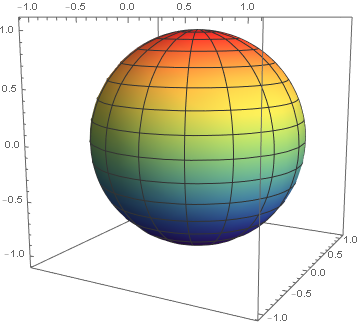
\includegraphics[width=.45\textwidth]{spz3d}
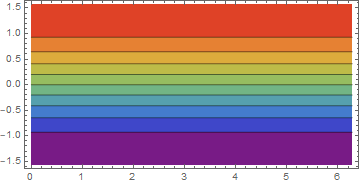
\includegraphics[width=.45\textwidth]{spzplane}
\caption{Representação gráfica da função $f(x,y,z) = z$ na esfera, tanto no espaço como no plano.} \label{spfunc}
\end{figure}
\end{ex}

\begin{ex}
De igual modo ao exercício anterior, represente a função $p(x,y,z) = x^2 - z^2$.
\end{ex}

\begin{ex}
Aplicando uma estratégia semelhante, represente no espaço e no plano as duas seguintes funções no toro:
\[g(x,y,z) = y; \quad h(u,v) = \cos(u) + \cos(v).\]

Nota: Poderá ter que re-escalar a função $h$ para a representar no espaço. Tenha também em atenção a opção \texttt{ColorFunctionScaling}.
\end{ex}


\end{document}